%---- fase design ----------------------------------------%
%
% \chapter{ESPECIFICAÇÃO FUNCIONAL}
% \label{chap:espfunc}

% %---- fase design ----------------------------------------
% \section{Funcionalidade}
% \label{sec:func1}

% %---- fase design ----------------------------------------
% \subsection{Descrição}
% \label{sec:desc1}

% %---- fase design ----------------------------------------
% \subsection{Premissas necessárias}
% \label{sec:prem1}

% %---- fase design ----------------------------------------
% \subsection{Dependências}
% \label{sec:dep1}

% %---- fase design ----------------------------------------
% \subsection{Saídas}
% \label{sec:said1}


\chapter{ANÁLISE ECONÔMICAx}
\label{chap:rsk}

%---- Análise de custos das operações com ROV ------------------------------------
\section{Análise de custos}
\label{sec:rskconc}
Os custos com operações offshore receberam limitada atenção dos meios acadêmico e corporativo. Em boa parte, os custos com a produção com petróleo e gás ocupam uma pequena porção orçamentária, além dos altos preços das commodities gerarem grandes fluxos de caixa, aumentando a produção e vendas por consequência (KAISER, 2019).

Diferente dos custos de capital para prospecção de petróleo e seus derivados, os custos operacionais são menos transparentes , com menor disponibilidade de dados e informações pertinentes para avaliação, vindo de diferentes formas e aplicações. Apesar de tais obstáculos, há estudos de benchmark que propuseram diminuir o gap entre as informações obtidas e a avaliação resultante do processo, obtendo relativo êxito em suas execuções. 

A proposta desta seção é avaliar os custos associados ao uso de manipuladores subaquáticos em ROVs. Para isso, os dados foram coletados e utilizados segundo informações da Petrobras a cerca dos contratos de embarcação de ROV para inspeção, reparo e manutenção, conforme apresentado na Tabela \ref{tab:cost1}:

\begin{table}[h!]
    \centering
	\begin{threeparttable}
	\centering
	\caption{Variáveis de embarcação tipo RSV}
	\label{tab:cost1}
    \begin{tabular}{p{8cm} >{\centering\arraybackslash}m{3.7cm}}
    %\begin{tabular}{l c}
		\hline
		\multicolumn{1}{c}{\textbf{Variáveis}} & \textbf{Valores}\tnote{i}  \\ \hline
		Diária RSV                              & US\$81.474,45     \\
		Ciclo 28 dias                          & US\$2.281.284,60  \\
		Total contrato RSV                     & US\$44.667.552,47 \\
		Total dias de contrato                 & 547               \\
		&                   \\
		Total de operações (A)\tnote{ii}                 & 1976              \\
		Total de inspeções                     & 1337              \\
		Total de intervenções                  & 639               \\
		Número de anomalias (B)                & 432               \\
		Índice de anomalias (B/A)              & 21,86\%           \\ \hline
	\end{tabular}
\begin{tablenotes}
\item[i]{Valores monetários a US\$ correntes}
\item[ii]{Operações e anomalias tiveram seus valores projetados para um ciclo contratual de 547 dias.}
\end{tablenotes}
\end{threeparttable}
\end{table}


Pode-se observar que os contratos de embarcação tipo RSV (ROV Support Vessel) da Petrobras são realizados em ciclos de 28 dias\footnote{Há também outros contratos internacionais que estabelecem um dia útil de 12 horas de trabalho, com permissão máxima de inatividade do ROV de 30 horas por mês (KAISER, 2019).} , com 1 dia de manutenção e reparo de equipamentos, alcançando a diária aproximada de US\$ 81 mil\footnote{Alguns estudos empíricos registram taxas diárias para RSV entre 100 e 300 mil dólares, dependendo do tamanho da embarcação utilizada.}. O valor da diária inclui, além do afretamento, materiais, equipamentos, bens importados e tripulação. 

Para gerar efeitos comparativos mais precisos, e considerando o uso da embarcação por 24 horas, as atividades descritas nos conjuntos da Tabela 1 terão o valor da diária estabelecido em minutos. A ideia consiste em mensurar a participação de uma determinada atividade em relação ao total previsto em um dia completo de operações. 
Estabeleceu-se a divisão das operações por conjunto segundo o nível de complexidade inerente à sua realização, i.é., o Conjunto 1 pode demandar um tempo menor de execução se comparado aos Conjuntos 3 e 4, por exemplo. As médias apresentadas na tabela seguem a seguinte estrutura:

\begin{table}[h!]
    \centering
    \resizebox{\textwidth}{!}{
	\begin{threeparttable}
	\centering
	\caption{Variáveis de embarcação tipo RSV}
	\label{tab:cost1}
    \begin{tabular}{l >{\centering\arraybackslash}m{3.0cm} >{\centering\arraybackslash}m{3.0cm} >{\centering\arraybackslash}m{3.0cm}}
		\hline
        \textbf{Operação submarina\tnote{i}}           & \textbf{Frequência média mensal} & {\textbf{Sem automação (min)}} & \textbf{Com automação (min)} \\ \hline
		Conjunto 1                                     &                                  &                                &                              \\
		\hspace{3mm}Abertura e fechamento de válvulas  & 12                               & 10                             & 5                            \\
		\hspace{3mm}Colocação e retirada de hot stab   & 28                               & 10                             & 4                            \\
		\hspace{3mm}Uso de torque tool                 & 12                               & 15                             & 5                            \\
		Conjunto 2                                     &                                  &                                &                              \\
		\hspace{3mm}Instalação de \textit{tree cap}    & 5                                & 60                             & 30                           \\
		\hspace{3mm}Conexão de \textit{flying leads}   & 10                               & 60                             & 15                           \\
		Conjunto 3                                     &                                  &                                &                              \\
		\hspace{3mm}Limpeza de \textit{hub}\tnote{ii}  & 5                                & 240                            & 60                           \\
		Conjunto 4                                     &                                  &                                &                              \\
		\hspace{3mm}Instalação de flanges              & 5                                & 180                            & 60                           \\ \hline
	\end{tabular}
    \begin{tablenotes}
        \item[i]{Valores monetários a US\$ correntes}
        \item[ii]{Operações e anomalias tiveram seus valores projetados para um ciclo contratual de 547 dias.}
    \end{tablenotes}
    \end{threeparttable}
    }
\end{table}

A hipótese central para os valores presentes no item C está em aproximar mais precisamente os tempos de execução das atividades presentes nos registros dos melhores condutores dos manipuladores. Por mais que estes tenham a experiência para uma boa condução, ainda há fatores (sejam eles de caráter endógeno ou exógeno) que possibilitam a presença de anomalias, enquanto com a automação estas seriam minimizadas.

O conjunto 1 corresponde às atividades que envolvem acionamento mecânico de válvulas submarinas com o ROV equipado com ferramentas de torque (\textit{torque tool}). Tal conjunto relaciona-se com os demais porque estes dependem diretamente do acionamento de válvulas para que ocorra a instalação/desinstalação de determinados equipamentos, o que justifica a maior frequência de manuseios de válvulas e \textit{torque tools}. Apesar de a Petrobras estabelecer máximo de 15 minutos para movimentos envolvendo válvulas, há registros apontando para valores médios de 10 minutos, com aproximação da média com automação em 5 minutos, uma diminuição de aproximadamente 50\% em relação à média máxima esperada em contrato.

O lançamento/instalação de \textit{Tree Cap} em árvore de natal molhada (ANM) e manuseio de \textit{flying leads}, utilizando ferramenta de torque, compõem o conjunto 2 de serviços do ROV. O principal diferencial para diminuição do tempo de execução em \textit{flying leads} está na presença de uma ferramenta de orientação inserida (FLOT) no ROV para colocá-los na ANM, que pode chegar em até 1/3 do valor comparado ao FLOT não residente. Para fins didáticos, o estudo propôs trabalhar somente com os valores onde há a utilização da ferramenta de orientação, registrando um total de execução de 60 minutos entre instalação e desinstalação dos componentes.

A operação de limpeza de \textit{hubs}, atividade fundamental do Conjunto 3, consiste em remover incrustações e/ou vidas marinhas dos equipamentos a partir de ferramentas de limpeza operadas por ROVs a fim de permitir instalação de subequipamentos. Em certas ocasiões, a limpeza do \textit{hub} está associada à necessidade de retirar as capas de proteção ou capas de teste. Por este motivo, quando realizadas no mesmo período programado, desinstalações de \textit{tree caps} (Conjunto 2) podem interferir diretamente no tempo de execução da limpeza do \textit{hub}, apresentando a maior média de tempo dentre todos os conjuntos de atividades no estudo. Ademais, a atividade em si depende muito da experiência do condutor do ROV e, dentro dos relatos da Petrobras, possui as maiores probabilidades de apresentar anomalias, gerando maiores desvios padrões em relação à média observada. Os valores representados na Tabela 1 para tal conjunto são equivalentes ao tempo médio de somente a realização da limpeza (4 horas aproximadamente).  

Por fim, o Conjunto 4 consiste na instalação de flanges cego (ou cubo cego \textit{grayloc}\footnote{Tecnologia desenvolvida por Oceaneering. Para mais informações, ver: https://www.oceaneering.com/grayloc-technology (acesso em 29/10/2019).}) em conexões de dutos rígidos e flexíveis, a partir de materiais fornecidos pela Petrobras. O conjunto envolve preparação e manuseio do flange no convés, lançamento, instalação de estojos, torqueamento e teste de estaqueidade. Dentro das atividades previstas, a instalação de estojos é a que possui maior interdependência entre os outros conjuntos de atividades descritas anteriormente, envolvendo inspeção visual, limpeza, destorqueamento, medição de potencial eletroquímico, instalação e torqueamento do novo estojo. Desta forma, torna-se mais complexa\footnote{Parte dessa complexidade também diz respeito ao uso correto da ferramenta, que deve possuir \textit{handles} em múltiplas posições para facilitar o manuseio pelo manipulador do ROV.}  a mensuração da performance. Para este estudo, a média de tempo para execução adotada foi de 180 minutos, podendo apresentar o mesmo comportamento observado no Conjunto 3.  

Dada a apresentação da estrutura dos conjuntos de atividades com manipuladores de ROV, deu-se prosseguimento à conversão dos dados em unidades monetárias para mensurar as proporções desses custos em relação à diária da embarcação, considerando para o caso somente as operações de intervenção\footnote{Apesar de haver uso de manipuladores para inspeções para casos de limpeza e medição de potencial eletroquímico, sua mensuração em tempo de execução é mais assertiva em inspeções programadas.}. Essa elaboração pode ser observada na Tabela 2, com os valores aproximados por minuto de uma diária completa de atividades, isto é, 24 horas (ou 1440 minutos) ininterruptas de prestação de serviço. 

\begin{table}[h!]
	\centering
	\caption{Dados monetários dos conjuntos de atividades em ROV}
	\label{tab:cost3}
	\def\arraystretch{1.2}
	\resizebox{\textwidth}{!}{%
		\begin{tabular}{llccc}
			\hline
            \multicolumn{2}{c}{\textbf{Operação submarina}} & \textbf{\begin{tabular}[c]{@{}c@{}}Valor médio de execução (US\$) \\ (A)\end{tabular}} & \textbf{\begin{tabular}[c]{@{}c@{}}Valor esperado com automação \\ (B)\end{tabular}} & \textbf{\begin{tabular}[c]{@{}c@{}}$\Delta$ A/B \\ (\%)\end{tabular}} \\ \hline
			\multicolumn{2}{l}{Conjunto 1}                  & \multicolumn{1}{l}{}                                                                   & \multicolumn{1}{l}{}                                                                 & \multicolumn{1}{l}{}                                          \\
			& Abertura e fechamento de válvulas      & 6.789,54                                                                               & 3.394,77                                                                             & 50\%                                                          \\
			& Colocação e retirada de hot stab       & 15.842,25                                                                              & 6.336,90                                                                             & 60\%                                                          \\
			& Uso de torque tool                     & 10.184,31                                                                              & 3.394,77                                                                             & 67\%                                                          \\
			\multicolumn{2}{l}{Conjunto 2}                  &                                                                                        &                                                                                      &                                                               \\
			& Instalação de tree cap                 & 16.973,84                                                                              & 8.486,92                                                                             & 50\%                                                          \\
			& Conexão de flying leads                & 33.947,69                                                                              & 8.486,92                                                                             & 75\%                                                          \\
			\multicolumn{2}{l}{Conjunto 3}                  &                                                                                        &                                                                                      &                                                               \\
			& Limpeza de hub                         & 67.895,38                                                                              & 16.973,84                                                                            & 75\%                                                          \\
			\multicolumn{2}{l}{Conjunto 4}                  &                                                                                        &                                                                                      &                                                               \\
			& Instalação de flanges                  & 50.921,53                                                                              & 16.973,84                                                                            & 67\%                                                          \\ \hline
		\end{tabular}%
	}
\end{table}
Observando os dados oriundos da Tabela 2, nota-se que as argumentações anteriormente apresentadas corroboram com os valores monetários expressos, sobretudo na interdependência dos Conjuntos 3 e 4 em relação às atividades mais ordinárias. É evidente que os dados apresentem proporções diretas com o presente na Tabela 1, visto que foram multiplicados por um valor constante (valor da diária de embarcação por minuto), o que justifica as variações percentuais entre 50 e 75\% das médias sem e com intermédio da automação, respectivamente.

Ademais, pode-se esperar margens ainda maiores com as atividades que possuem tempos de execução com alto desvio-padrão, como é o caso da instalação de \textit{tree cap} e da limpeza de \textit{hub}. 

Ao realizar a soma dos valores monetários dos conjuntos, obtêm-se algumas importantes observações e desdobramentos, que podem ser verificados na Tabela 3.

\begin{table}[h!]
	\centering
	\caption{Soma dos custos das atividades com manipuladores}
	\label{tab:cost4}
	\def\arraystretch{1.2}
	\resizebox{\textwidth}{!}{%
		\begin{tabular}{llll}
			\hline
			\textbf{Conjunto de Operações} & \textbf{Valor sem automação (A)} & \textbf{Valor com automação (B)} & \textbf{Redução (A - B)} \\ \hline
			Conjunto 1                     & 32.816,10                        & 13.126,44                        & 19.689,66                \\
			Conjunto 2                     & 50.921,53                        & 16.973,84                        & 33.947,69                \\
			Conjunto 3                     & 67.895,38                        & 16.973,84                        & 50.921,53                \\
			Conjunto 4                     & 50.921,53                        & 16.973,84                        & 33.947,69                \\
			\textbf{Total}                 & \textbf{202.554,54}              & \textbf{64.047,97}               & \textbf{138.506,57}      \\ \hline
		\end{tabular}%
	}
\end{table}

Com os valores monetários expressos na Tabela 3, espera-se que haja uma redução de custos de aproximadamente 59\%  \footnote{O percentual não englobou os custos associados a pessoal e logística, assim como a depreciação, reparos e manutenções necessárias.}em relação aos conjuntos de operações realizados sem automação. Visto que são valores representativos a duas instalações simultâneas em árvores de natal molhada por mês, esses podem obter um impacto ainda mais significativo se analisado em período anual.

Além dos impactos diretos nos custos com as operações dos manipuladores, outros possíveis efeitos indiretos devem ser considerados como, por exemplo, a minimização de anomalias em riscos ambientais e diminuição do consumo de óleo diesel, necessário para o funcionamento das embarcações de ROVs. 

Por fim, vale destacar a importância de um conjunto de atividades específicas ao monitoramento sísmico marítimo utilizando receptores pontuais (também conhecidos como \textit{nodes}). 

Por ser uma tecnologia disruptiva, pioneira no âmbito mundial, ela servirá para gerenciamento da produção dos reservatórios do Pré-Sal da Bacia de Santos. As hipóteses para sua implementação são os ganhos de qualidade intrínseca dos dados sísmicos - incluindo qualidade sísmica 4D - e ganhos de tempo de processamento destes dados. Além da maior flexibilidade operacional e qualidade dos dados, o conceito terá uma rápida capacidade de apropriação pela Petrobras, uma vez que a tecnologia já está madura e amplamente desenvolvida na empresa\footnote{Um exemplo desse domínio são as estacas-torpedos, empregadas como meio de baixo custo para enterramento dos \textit{nodes}.}.

As etapas previstas para as quais a tecnologia deverá passar são: 

\begin{itemize}
	\item Prototipagem, que inclui a produção de uma maquete em escala reduzida;
	\item Validação dos componentes e do sistema em escala laboratorial, ainda na fase de P\&D;
	\item Testes em escala reduzida, ambiente controlado e incluindo a estaca instrumentada;
	\item Produção de cinco unidades constituídas de um Módulo Submarino de Aquisição de Dados Sísmicos (MSADS) e um Dispositivo de Transporte e Liberação de Estacas (DLTE);
	\item Teste de campo para validação da operação em condições realistas;
	\item Avaliação da prova de conceito final e recomendações para manufatura em escala comercial.
\end{itemize}

A justificativa para tal conceito estar dentro do estudo encontra-se nas operações do ROV com o Módulo de Estaca-Suporte (MES), MSADS, Módulo de Posicionamento e Alinhamento (MPA), sendo estas necessárias tanto para operações de instalação quanto de desinstalação dos componentes, cujos tempos de execução sem a automação e os previstos com a implementação da automação dos manipuladores podem ser observados na Tabela 4.

\begin{table}[h!]
	\centering
	\caption{Tempos de execução com operações do MSADS}
	\label{tab:node1}
	\def\arraystretch{1.2}
	\resizebox{\textwidth}{!}{%
		\begin{tabular}{llcc}
			\hline
			& \textbf{}                                                          & \multicolumn{2}{c}{\textbf{Duração}}                                                                                                    \\ \hline
			& \multicolumn{1}{c}{\textbf{Etapa/Descrição}}                       & \textbf{\begin{tabular}[c]{@{}c@{}}Manual \\ (min)\end{tabular}} & \textbf{\begin{tabular}[c]{@{}c@{}}Automático \\ (min)\end{tabular}} \\ \hline
			\multicolumn{2}{l}{Instalação}                                        & \multicolumn{1}{l}{}                                             & \multicolumn{1}{l}{}                                                 \\
			& Posicionar o MSADS no disco da estaca                              & 12                                                               & 5                                                                    \\
			& Retirar capa protetora do conector elétrico e colocá-la no suporte & 14                                                               & 6                                                                    \\
			& Retirar conector elétrico no jumper e colocar em painel de estaca  & 15                                                               & 6                                                                    \\
			\multicolumn{2}{l}{Desinstalação}                                     &                                                                  &                                                                      \\
			& Desconectar do jumper do painel e colocar o conector elétrico      & 12                                                               & 5                                                                    \\
			& Recolocar a capa protetora no painel de estaca                     & 14                                                               & 6                                                                    \\
			& Retirar o MSADS do disco da estaca                                 & 11                                                               & 4                                                                    \\ \hline
		\end{tabular}%
	}
\end{table}

As etapas das operações que necessitam do auxílio do ROV consistem em lançar várias estacas-suporte em ambiente submarino, conectar os módulos permanentes e não-permanentes, registro sísmico, desconexão do módulo de eletrônica e recuperação dos dados registrados.  

O MSADS, também conhecido como Módulo de Eletrônica, contém um suporte para que este seja suspenso por um ROV, além de um conector de conexão molhada, manuseável pelo manipulador presente no veículo, para colocá-lo ao painel da Estaca-suporte. 

Inicialmente posiciona-se o MSADS no disco de estaca, procedimento que leva em média 12 minutos para execução. Em seguida, retira-se a capa protetora do conector elétrico no painel da estaca e coloca essa em seu suporte no painel, com uma estimativa de execução de aproximadamente 14 minutos. Compondo a etapa final de instalação, há a retirada do conector elétrico na extremidade do \textit{jumper}\footnote{Operações de conexões e desconexões de \textit{jumper} elétrico consistem em realizar interligações/desconexões elétrica entre equipamentos e/ou subequipamentos submarinos com a finalidade de permitir comando e monitoramento eletroeletrônico a partir da superfície.}  no MSADS e realiza-se a conexão deste no painel da estaca, com tempo estimado de 15 minutos para realização. Espera-se que, com a automação dos manipuladores, haja uma redução média de 24 minutos entre todas as operações de instalação.

Para os processos de desinstalação, de início, a primeira etapa consiste em desconectar o \textit{jumper} do painel da estaca e colocar o conector elétrico do \textit{jumper} em seu suporte no Módulo de Eletrônica, com duração aproximada de 12 minutos. A etapa seguinte procura recolocar a capa protetora no conector elétrico do painel da Estaca-suporte, levando em média 14 minutos para sua execução. Por fim, realiza-se a operação de retirada do MSADS do disco de estaca por volta de 11 minutos. Da mesma maneira que nas instalações, com a automação espera-se que haja uma redução total cerca de 22 minutos.

\begin{table}[h!]
	\centering
	\caption{Valores das atividades realizadas com nodes}
	\label{tab:node2}
	\def\arraystretch{1.2}
	\resizebox{\textwidth}{!}{%
		\begin{tabular}{llccc}
			\hline
			&                                                       & \multicolumn{3}{c}{\textbf{Valores (diária)}}                                                                                                                                                                   \\ \hline
			& \multicolumn{1}{c}{\textbf{Etapa/Descrição}}          & \textbf{\begin{tabular}[c]{@{}c@{}}Manual (US\$) \\ (A)\end{tabular}} & \textbf{\begin{tabular}[c]{@{}c@{}}Automático (US\$)\\ (B)\end{tabular}} & \textbf{\begin{tabular}[c]{@{}c@{}}A/B \\ (\%)\end{tabular}} \\ \hline
			\multicolumn{2}{l}{Instalação}                           & \multicolumn{1}{l}{}                                                  & \multicolumn{1}{l}{}                                                     & \multicolumn{1}{l}{}                                         \\
			& Posicionamento do MSADS no disco da estaca            & 1.250,00                                                              & 520,83                                                                   & 58,33                                                        \\
			& Retirar e colocar capa protetora do conector elétrico & 1.458,33                                                              & 625,00                                                                   & 57,14                                                        \\
			& Retirar e colocar conector elétrico no jumper         & 1.562,50                                                              & 625,00                                                                   & 60,00                                                        \\
			\multicolumn{2}{l}{Desinstalação}                        &                                                                       &                                                                          &                                                              \\
			& Desconectar do jumper e colocar o conector elétrico   & 1.250,00                                                              & 520,83                                                                   & 58,33                                                        \\
			& Recolocar a capa protetora no conector elétrico       & 1.458,33                                                              & 625,00                                                                   & 57,14                                                        \\
			& Retirar o MSADS do disco da estaca                    & 1.145,83                                                              & 416,67                                                                   & 63,64                                                        \\ \hline
		\end{tabular}%
	}
\end{table}
De maneira análoga ao apresentado nas Tabelas 2 e 3, os dados dos tempos de execução em operações com os módulos submarinos foram multiplicados por um valor da diária de embarcação proporcional por minuto. Para operações como essas, a embarcação mais adequada é a de pesquisa sísmica, cujo valor adotado foi de US\$161,9 mil\footnote{Tanto em relatórios anuais das empresas prestadoras de serviços quanto a literatura acadêmica empírica utilizam de uma margem que, para os valores correntes, chegam entre US\$150 e US\$200 mil.} , e que pode ser observado na Tabela 5. 

As variações percentuais presentes na última coluna corroboram a importância da automação nos processos envolvendo monitoramento sísmico\footnote{Vale ressaltar que a instalação do Módulo de Posicionamento e Alinhamento (MPA) também pode ser autônomas. Para tal, espera-se que haja uma redução de 2 minutos, em média, entre as operações sem e com automação. Por ser uma oportunidade tecnológica em fase de exploração pela Petrobras, não há dados monetários concretos para serem levantados.}. Por   permanente. Os valores monetários expressos podem ainda sofrer alterações significativas dependendo da diária estabelecida em contrato, dentro dos padrões internacionais para este tipo de atividade. Quando representados em um período contratual de uma embarcação de pesquisa sísmica, as operações elucidadas na Tabela 5 possuem amplas margens de redução de custo com a automação.

\begin{table}[h!]
	\centering
	\caption{Valores proporcionais em período de contratação - nodes}
	\label{tab:node3}
	\def\arraystretch{1.2}
	\resizebox{\textwidth}{!}{%
		\begin{tabular}{lllll}
			\hline
			\multicolumn{1}{c}{\textbf{Tipo de operação}} & \multicolumn{1}{c}{\textbf{\begin{tabular}[c]{@{}c@{}}Manual (US\$ 1000) \\ mín\end{tabular}}} & \multicolumn{1}{c}{\textbf{\begin{tabular}[c]{@{}c@{}}Automático (US\$ 1000) \\ mín\end{tabular}}} & \multicolumn{1}{c}{\textbf{\begin{tabular}[c]{@{}c@{}}Manual (US\$ 1000) \\ máx\end{tabular}}} & \multicolumn{1}{c}{\textbf{\begin{tabular}[c]{@{}c@{}}Automático (US\$ 1000) \\ máx\end{tabular}}} \\ \hline
			Instalação                                    & 4.609,47                                                                                       & 1.911,24                                                                                           & 27.656,81                                                                                      & 11.467,46                                                                                          \\
			Desinstalação                                 & 4.159,76                                                                                       & 1.686,39                                                                                           & 24.958,58                                                                                      & 10.118,34                                                                                          \\
			\textbf{Total}                                & \textbf{8.769,23}                                                                              & \textbf{3.597,63}                                                                                  & \textbf{52.615,39}                                                                             & \textbf{21.585,80}                                                                                 \\
			\textbf{Diferença}                            & \textbf{-}                                                                                     & \textbf{5.171,60}                                                                                  & \textbf{-}                                                                                     & \textbf{31.029,59}                                                                                 \\ \hline
		\end{tabular}%
	}
\end{table}

Quando agregadas as atividades de instalação e desinstalação dos Módulos de Eletrônica, a redução de custo pode variar de 5,2 a 31 milhões de dólares por contrato. A justificativa para o desvio padrão apresentado está na quantidade de intervenções já realizadas até então pela Petrobras por ciclos contratuais. Ademais, tal desvio padrão viabiliza as oportunidades tecnológicas presentes na automação do monitoramento sísmico, com o escopo de 2 anos e meio para tornar o sistema no mínimo semi-operacional.

Em suma, do ponto de vista financeiro, espera-se que a automação provenha reduções significativas de custos associadas aos manipuladores de ROV, seja em operações mais ordinárias, como aberturas e fechamentos de válvulas, seja em operações onde a Petrobras obterá o pioneirismo mundial, como nas operações de intervenções em \textit{nodes all-in-two}. 

Entretanto, para que a automação dos manipuladores seja considerada viável no âmbito econômico, verificou-se a necessidade de se avaliar a rentabilidade dos projetos de P\&D associados, em uma metodologia de valoração amplamente utilizada por empresas e academia, e que será explorada na seção seguinte. 


%---- Modelo de Valoração P&D ----------------------------------------
\section{Modelo de valoração dos projetos de P\&D}
\label{sec:rskdesig}

A fim de obterem vantagens competitivas que proporcionem lucros monopolísticos\footnote{A busca de oportunidades ou inovação, em seu sentido mais amplo, geram monopólios temporários, de menor ou maior período, até que sejam desafiados por novos concorrentes ou imitadores, tornando a concorrência um processo ativo e evolutivo de espaço e oportunidades tecnológicos. Para mais, ver Possas(2005).} , as empresas buscam inovações e o mercado, consequentemente, selecionam os resultados econômicos oriundos dessas mesmas inovações através de decisões estratégicas. 

Essas estratégias podem ocorrer através de investimentos em P\&D, atuando como ativos intangíveis e cujos esforços convertem-se em desenvolvimento de novos produtos, processos e/ou serviços. Os resultados deste processo são observáveis através dos impactos gerados na esfera empresarial, ou até mesmo no âmbito socioeconômico. 

No entanto, como discutido na introdução, os esforços para se investir em P\&D possuem incertezas inerentes que tornam a atividades de difícil avaliação ex-ante. Para isso, a Teoria de Opções Reais apresenta-se como um método robusto para análises de cenários onde há presença de incerteza e flexibilidade gerencial de longo prazo (DIXIT \& PYNDICK, 1994; MUN, 2002). 

Considerando que todo projeto de P\&D é, em essência, um projeto de investimento produtivo, este pode ser visto como um conjunto de opções reais. Dentre tais opções, as empresas detêm a capacidade de optar de adiar o investimento, cancelar novas etapas, alterar a escala produtiva (como é o caso de expansão e contração), abandonar por conta do excessivo ônus e opções de crescimento (MEIRELLES, 2004). 

Para a construção da análise, utilizaram-se dados provenientes da última demonstração financeira da Petrobras e dos esforços de P\&D, que estarão concentrados integralmente nos recursos alocados e esperados em parceria com o SENAI CIMATEC, e que podem ser observados na Tabela 6.

\begin{table}[h!]
	\centering
	\caption{Variáveis utilizadas para modelo de valoração}
	\label{tab:valor1}
	\def\arraystretch{1.2}
	\begin{tabular}{lc}
		\hline
		\multicolumn{1}{c}{\textbf{Variáveis}} & \textbf{Valor} \\ \hline
		Investimento na Fase 1                 & R\$ 1,34 mi    \\
		Investimento na Fase 2                 & R\$ 18 mi      \\
		VPL descontado                         & R\$ 20,23 mi   \\
		Volatilidade                           & 25\%           \\
		Taxa risk-free                         & 5\%            \\
		Período da Fase 1                      & 1 ano          \\
		Período da Fase 2                      & 2 anos         \\ \hline
	\end{tabular}
\end{table}

O investimento para o projeto foi dividido em duas grandes fases: inicialmente, o desenvolvimento viável das provas de conceito para, em seguida, testar o desempenho da automação dos manipuladores em ambientes reais. Para isso, estima-se investimentos de aproximadamente R\$ 19,34 milhões em um período de 3 anos. Utilizando a simulação Monte Carlo, e baseado na convergência das respostas dos pesquisadores com a metodologia A$Dˆ2$ (Advancement Degree of Difficulty)\footnote{A metodologia baseia-se na mensuração das dificuldades previstas no projeto para amadurecer o uso da tecnologia. Variáveis como custo, cronograma e os riscos inerentes às fases do projeto são consideradas na avaliação.} , a volatilidade implícita dos fluxos de caixa esperados com o projeto é de 25\%. 

Para a valoração estática dos lucros futuros, utilizou-se o modelo de fluxos de caixa descontado por uma taxa de desconto baseada no custo médio ponderado sobre o capital. A partir dos dados provenientes das demonstrações financeiras, a Petrobras teve, em 2018, 290 propriedades intelectuais (em grande parte, patentes) concedidas no Brasil e exterior. O valor adicionado recebido em alugueis, royalties e outros por conta de tais propriedades ficou em torno de R\$1,1 bilhão. Constatando os valores adicionados em períodos anteriores e dividindo pelas patentes concedidas, calculou-se o valor de R\$2,62 milhões por concessão, que serviu para a elaboração dos fluxos de caixa descontados, obtendo o resultado esperado de R\$20,23 milhões. 

O cálculo da árvore inicial é similar às operações tradicionais de opções reais com ativos, calculando os fatores superiores e inferiores e envolvendo o valor presente dos fluxos de caixa futuros para os próximos três anos, presente na Figura \ref{fig:eco1}.

% \begin{figure}
% 	\centering
% 	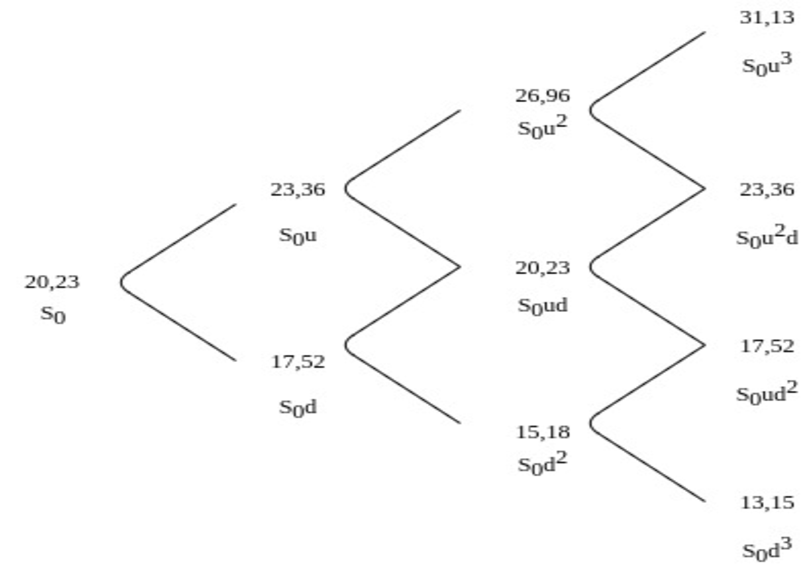
\includegraphics[width=.75\textwidth]{images/eco1.pdf}
% 	\caption{Construção inicial da árvore}
% 	\label{fig:eco1}
% \end{figure}

No entanto, espera-se que o projeto possua duas fases de desenvolvimento. Para isso, foi estabelecido a opção composta sequencial, que ocorre quando um projeto tem múltiplas fases e o andamento para etapas subsequentes dependem necessariamente do sucesso prévio. Realizando os cálculos para a construção dos nós da primeira e segunda etapa, além dos valores estimados com o objetivo de manter ou abandonar o projeto, a análise das opções combinadas pode ser visualizada na Figura \ref{fig:eco2}. 

Os valores presentes líquidos (VPL) dos futuros fluxos de caixa esperados na análise corroboram com os percentuais dos fatores superiores e inferiores. Ademais, a probabilidade de sucesso é alta, visto que a prova de conceito se mostrou viável no âmbito técnico e possui desdobramentos positivos para futuras etapas.

% \begin{figure}[h!]
% 	\centering
% 	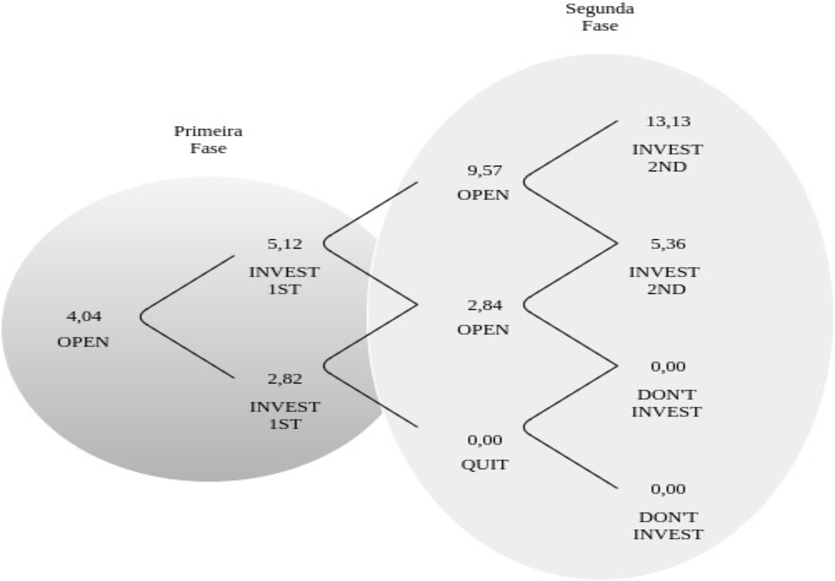
\includegraphics[width=.75\textwidth]{images/eco2.pdf}
% 	\caption{Construção inicial da árvore}
% 	\label{fig:eco2}
% \end{figure}

A resposta positiva à primeira fase, apresentada nos valores do primeiro nó, abrem a possibilidade de investimentos para uma segunda fase de desenvolvimento. Mesmo em um cenário mais desfavorável, os futuros fluxos de caixa possuem valores acima das etapas anteriores, o que demonstra uma gradativa evolução tanto do ponto de vista financeiro quanto técnico, no que diz respeito à apropriação da tecnologia de automação dos manipuladores.

Na segunda fase, apesar de apresentar a metade dos nós com VPL maiores que zero, o cenário é positivo para novas concessões com a propriedade intelectual gerada pelo projeto de P\&D em questão. Além disso, é importante reforçar que as árvores não se utilizaram de futuros fluxos de caixa e nem dos investimentos provenientes do monitoramento sísmico (\textit{nodes all-in-two}), o que poderia gerar externalidades positivas ainda mais significativas, uma vez que a empresa detém a apropriabilidade tecnológica dos nodes. 

Em síntese, é possível inferir que há retornos significativos com os esforços de P\&D a serem realizados nos períodos subsequentes. Evidentemente que a análise de Opções Reais possui limitações, como não considerar riscos associados a grandezas macroeconômicas, ou levar em consideração a volatilidade como uma constante ao longo do tempo. Porém, diante dos cenários apresentados e da capacidade de apropriação sobre a tecnologia, o horizonte para exploração de novas oportunidades sobre automação dos manipuladores submarinos é favorável.


%---- Conclusão ----------------------
\section{Conclusão análise econômica}
\label{sec:rskdesen}

A partir das análises efetuadas neste estudo, e do ponto de vista econômico, pode-se concluir que as hipóteses levantadas - reduções de custo de inspeção e intervenções com manipuladores de ROV, e ganhos de performance associados ao tempo de execução - foram corroboradas pelas significativas reduções tanto no tempo dos conjuntos de atividades quanto nos custos associados à realização destas, que apresentam valores entre 50 e 75\% dos desempenhos atuais com os condutores. 

Verificando o processo de valoração do projeto de P\&D em questão, o cenário é favorável para que se realize novos esforços inovativos, uma vez que será possível não somente apropriar-se da tecnologia disruptiva como também dos lucros monopolísticos associados à concessão da propriedade intelectual para terceiros, que, no melhor cenário possível, pode chegar a 3,25 vezes o VPL apresentado no início do projeto. 

Ao levar em consideração os custos associados com o monitoramento sísmico, as estimativas de redução são ainda mais otimistas se comparadas às atividades mais tradicionais realizadas com os manipuladores, ficando entre 57,14 e 63,64\% comparando com os valores sem automação. 

Por fim, faz-se uso de algumas possíveis recomendações para futuros desdobramentos destes estudos, como a valoração do projeto de monitoramento sísmico, avaliação \textit{ex-post} dos ganhos associados à automação dos manipuladores de ROV, e os possíveis desdobramentos com as oportunidades tecnológicas futuros no tema. 
